
%(BEGIN_QUESTION)
% Copyright 2010, Tony R. Kuphaldt, released under the Creative Commons Attribution License (v 1.0)
% This means you may do almost anything with this work of mine, so long as you give me proper credit

Suppose the voltmeter in this circuit is ``pegged'' in the negative direction (i.e. it registers a strong {\it negative} voltage beyond its normal measurement range).  A test using a digital multimeter (DMM) shows the voltage between test points {\bf D} and {\bf B} to be 6 volts:

$$\includegraphics[width=15.5cm]{i00329x01.eps}$$

Identify the likelihood of each specified fault for this circuit.  Consider each fault one at a time (i.e. no coincidental faults), determining whether or not each fault could independently account for {\it all} measurements and symptoms in this circuit.

% No blank lines allowed between lines of an \halign structure!
% I use comments (%) instead, so that TeX doesn't choke.

$$\vbox{\offinterlineskip
\halign{\strut
\vrule \quad\hfil # \ \hfil & 
\vrule \quad\hfil # \ \hfil & 
\vrule \quad\hfil # \ \hfil \vrule \cr
\noalign{\hrule}
%
% First row
{\bf Fault} & {\bf Possible} & {\bf Impossible} \cr
%
\noalign{\hrule}
%
% Another row
$R_1$ failed open &  &  \cr
%
\noalign{\hrule}
%
% Another row
$R_2$ failed open &  &  \cr
%
\noalign{\hrule}
%
% Another row
$R_3$ failed open &  &  \cr
%
\noalign{\hrule}
%
% Another row
$R_4$ failed open &  &  \cr
%
\noalign{\hrule}
%
% Another row
$R_1$ failed shorted &  &  \cr
%
\noalign{\hrule}
%
% Another row
$R_2$ failed shorted &  &  \cr
%
\noalign{\hrule}
%
% Another row
$R_3$ failed shorted &  &  \cr
%
\noalign{\hrule}
%
% Another row
$R_4$ failed shorted &  &  \cr
%
\noalign{\hrule}
%
% Another row
Voltage source dead &  &  \cr
%
\noalign{\hrule}
} % End of \halign 
}$$ % End of \vbox

Finally, identify the {\it next} diagnostic test or measurement you would make on this system.  Explain how the result(s) of this next test or measurement help further identify the location and/or nature of the fault.

\vfil 

\underbar{file i00329}
\eject
%(END_QUESTION)





%(BEGIN_ANSWER)

This is a graded question -- no answers or hints given!

%(END_ANSWER)





%(BEGIN_NOTES)

If all we knew about this circuit is that the voltmeter was ``pegged'' in the negative direction, then we would suspect up to {\it four} different possible faults that could unbalance the bridge circuit in this direction (those shown below, plus $R_2$ failed open or $R_1$ failed shorted.  However, we can narrow the range of possibilities down to just {\it two} faults because we have the 6 volt measurement between test points {\bf D} and {\bf B} which shows us that both $R_1$ and $R_2$ are functioning properly.  Therefore our fault table looks like this:

% No blank lines allowed between lines of an \halign structure!
% I use comments (%) instead, so that TeX doesn't choke.

$$\vbox{\offinterlineskip
\halign{\strut
\vrule \quad\hfil # \ \hfil & 
\vrule \quad\hfil # \ \hfil & 
\vrule \quad\hfil # \ \hfil \vrule \cr
\noalign{\hrule}
%
% First row
{\bf Fault} & {\bf Possible} & {\bf Impossible} \cr
%
\noalign{\hrule}
%
% Another row
$R_1$ failed open &  & $\surd$ \cr
%
\noalign{\hrule}
%
% Another row
$R_2$ failed open &  & $\surd$ \cr
%
\noalign{\hrule}
%
% Another row
$R_3$ failed open & $\surd$ &  \cr
%
\noalign{\hrule}
%
% Another row
$R_4$ failed open &  & $\surd$ \cr
%
\noalign{\hrule}
%
% Another row
$R_1$ failed shorted &  & $\surd$ \cr
%
\noalign{\hrule}
%
% Another row
$R_2$ failed shorted &  & $\surd$ \cr
%
\noalign{\hrule}
%
% Another row
$R_3$ failed shorted &  & $\surd$ \cr
%
\noalign{\hrule}
%
% Another row
$R_4$ failed shorted & $\surd$ &  \cr
%
\noalign{\hrule}
%
% Another row
Voltage source dead &  & $\surd$ \cr
%
\noalign{\hrule}
} % End of \halign 
}$$ % End of \vbox

Given the fault possibilities of $R_3$ open or $R_4$ shorted, there are no more voltage tests that will help us pinpoint the fault.  Measuring voltage across either $R_3$ or across $R_4$ will tell us nothing new: if $R_3$ is open then it will drop 12 volts and $R_4$ will drop 0 volts; if $R_4$ is shorted then it will drop 0 volts and $R_3$ will drop 12 volts.

A good test we could do, however, is measure total {\it current} through the circuit, knowing any open fault will result in a less-than-normal total current while any shorted fault will result in a greater-than-normal total current.

%INDEX% Troubleshooting review: electric circuits (Wheatstone bridge)

%(END_NOTES)

